% !TeX spellcheck = it_IT
% !TEX TS-program = pdflatex
% !TEX root = ../main.tex


% ********************************************************************
\section{Prototipo}
\label{sec:prototipo}
% ********************************************************************


\subsection{Login e autenticazione}

\subsubsection{Ente}



\subsubsection{Donatore}



\subsection{Dashboard donatore}
La \textit{dashboard} del donatore è l'interfaccia attraverso la quale gli utenti possono interagire direttamente con la piattaforma a seguito della procedura di autenticazione. 


Considerata la natura dei proponenti (Enti del terzo settore e \gls{onp}), il sistema implementa il meccanismo di raccolta del \textit{Keep-it-all}, secondo cui l'ente beneficiario trattiene i fondi raccolti anche qualora l'obiettivo non venga raggiunto entro i termini prefissati.


\begin{figure}[h]
	\centering
	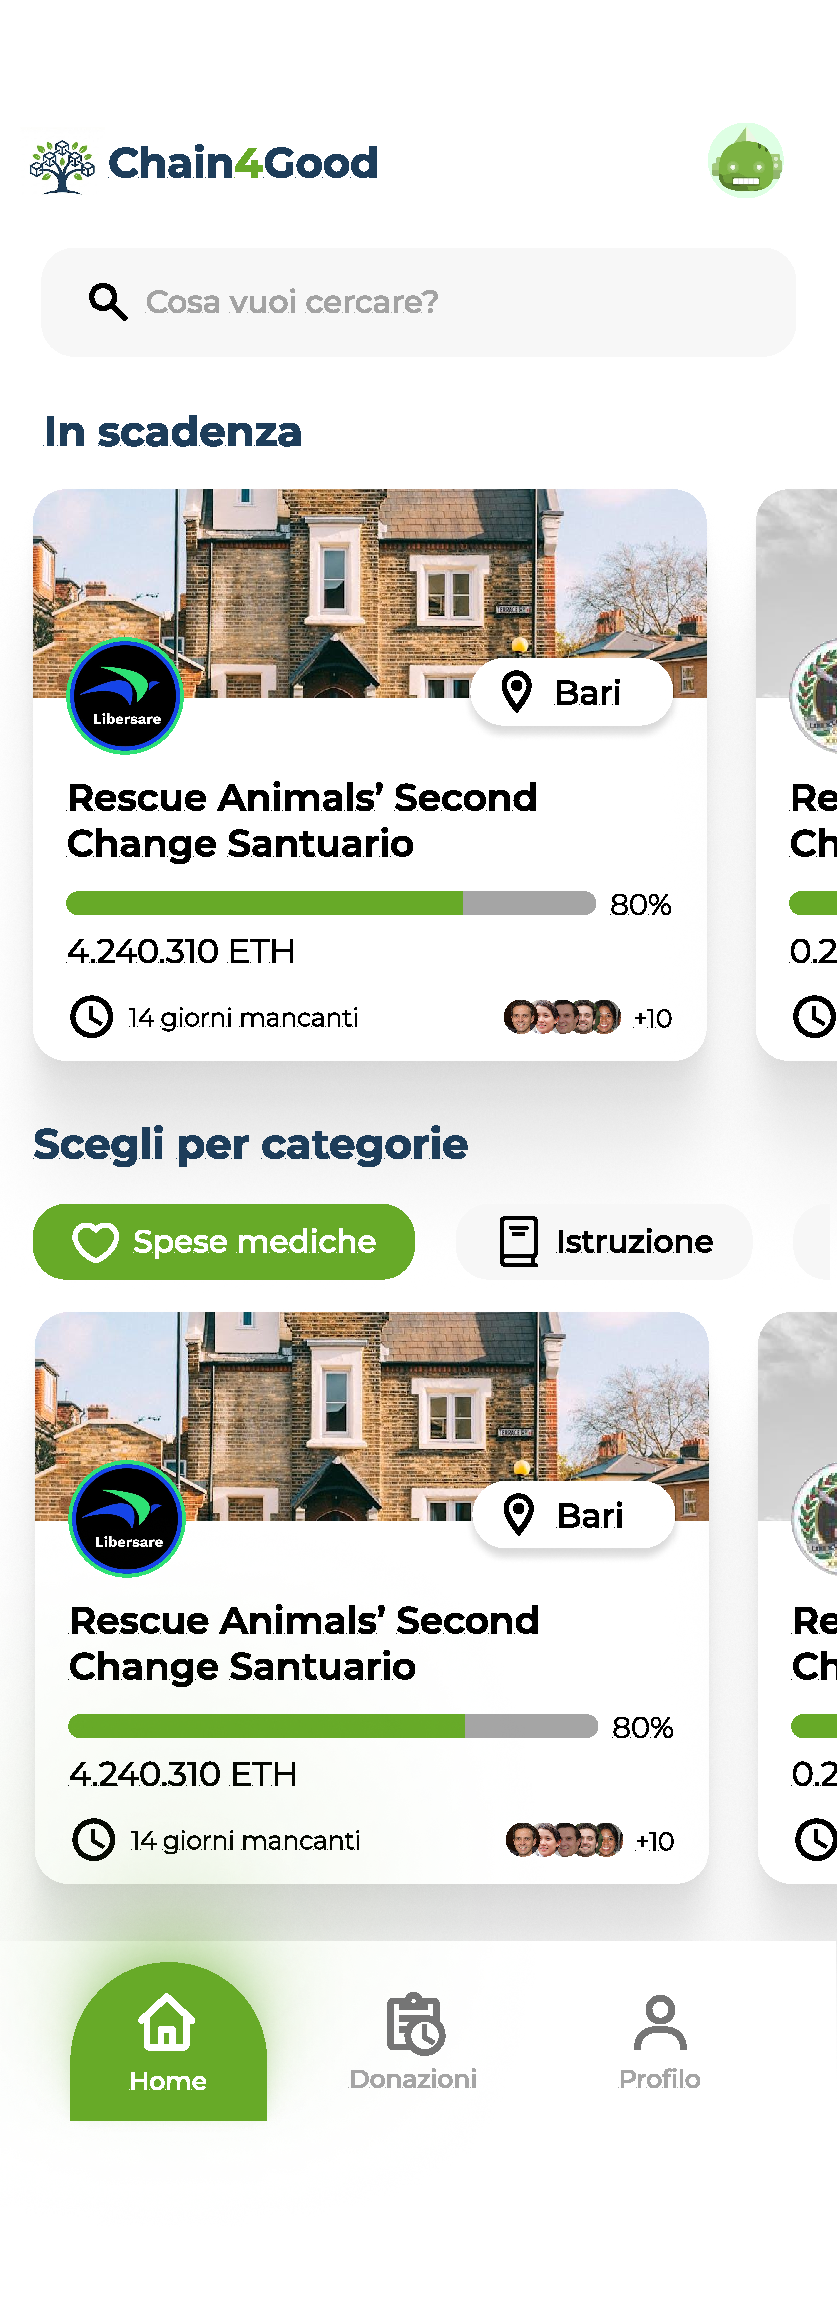
\includegraphics[width=0.45\textwidth]{images/home_utente.pdf}
	\caption{Dashboard del donatore}
	\label{fig:dashboard-donatore}
\end{figure}



\subsection{Creazione progetto}




\begin{figure}[h]
	\centering
	\begin{minipage}{0.46\textwidth}
		\centering
		\includegraphics[width=\textwidth]{images/nuovo_progetto1.pdf}
	\end{minipage}
	\hspace{0.9cm}
	\begin{minipage}{0.46\textwidth}
		\centering
		\includegraphics[width=\textwidth]{images/nuovo_progetto2.pdf}
	\end{minipage}
	\caption{Inserimento di un nuovo progetto}
	\label{fig:Inserimento progetto}
\end{figure}





\subsection{Inserimento e valutazione spesa}

A differenza dei sistemi centralizzati in cui l'Ente ha piena e immediata disponibilità del \textit{budget} donato, l’architettura proposta prevede che i fondi raccolti rimangano vincolati all'interno di uno \textit{Smart Contract}. \\
Per accedere a tali risorse, il beneficiario deve formalizzare una "Richiesta di Spesa" (\ref{fig:valutazione-spesa}) attraverso l'inserimento dei seguenti parametri: identificativo della spesa, importo richiesto, finalità dell'esborso e preventivo. \\
Una volta sottomessa la richiesta, la piattaforma permette ai donatori di analizzare la documentazione ed esercitare il proprio diritto di voto.

\begin{figure}
	\centering
	\begin{minipage}{0.46\textwidth}
		\centering
		\includegraphics[width=\textwidth]{images/nuova_spesa.pdf}
	\end{minipage}
	\hspace{0.9cm}
	\begin{minipage}{0.40\textwidth}
		\centering
		\includegraphics[width=\textwidth]{images/valutazione_spesa.pdf}
	\end{minipage}
	\caption{Valutazione di una richiesta di spesa}
	\label{fig:valutazione-spesa}
\end{figure}

\subsubsection{Meccanismo di validazione}
Per garantire l'operatività del sistema ed evitare lo stallo decisionale, lo \textit{Smart Contract} è stato programmato per agire secondo le seguenti regole:
\begin{itemize}
	\item La richiesta è approvata se la maggioranza dei votanti (rappresentata dalla comunità di individui che finanzia un'iniziativa) esprime un parere favorevole. In presenza di una partecipazione parziale, la soglia di maggioranza viene ricalcolata in funzione dei soli voti espressi.
	\item Qualora non venga registrata alcuna attività di voto, il sistema approva automaticamente la richiesta.
\end{itemize}

Al soddisfacimento dei requisiti di approvazione, lo \textit{Smart Contract} esegue in modo autonomo e irreversibile il trasferimento della somma raccolta verso il \textit{Wallet} del beneficiario. 

